\section{Auswertung}
\begin{figure}
    \centering
    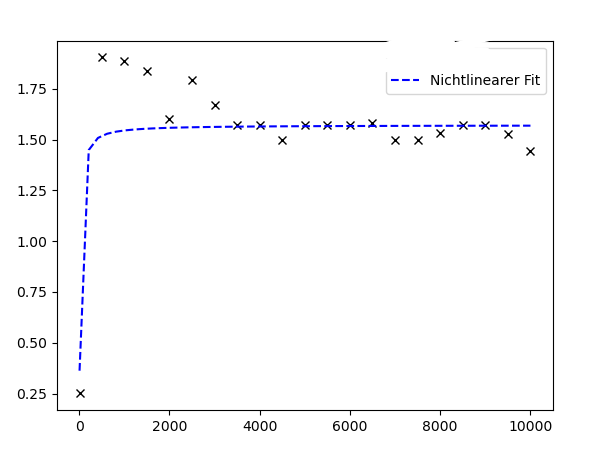
\includegraphics[width=0.6\textwidth]{build/plot1.pdf}
    \caption{Schematischer Aufbau des Lock-In-Verstäker mit installiertem Photodetektor. \cite{skript}} 
    \label{fig:licht}
\end{figure}

Untersucht wurden die Ausgangsspannungen am Lock-In-Verstäker in Abhängigkeit von dem Phasenunterschied zwischen Signal- und Referenzspannung. Im Folgenden ist die Auswertung 
für eine Signalspannung mit und ohne Rauschen unterteilt.

\subsection{Ausgangsspannung ohne Rauschen}
In diesem Versuchsteil wurden die Ausgangsspannungen am Lock-In-Verstäker einer mit einer Rechteckspannung modifizierten sinusförmigen Signalspannung gemessen. In der Tabelle ..
sind die Ausgangsspannung $U_{\text{out}}$ in Abhängigkeit von der Phase notiert. An einem Oszilloskop ließen sich Momentanaufnahmen von Signalspannung (in Gelb), sowie den Ausgangsspannungen in Türkis anfertigen.
Die Abbildungen \ref{fig:11} bis \ref{fig:18} zeigen die Spannungen in Abhängigkeit von der Phase $\phi$ welche von $\SI{0}{\degree}$ bis $\SI{360}{\degree}$ verändert werden.
\begin{figure}
    \begin{minipage}{0.5\textwidth}
        \centering
        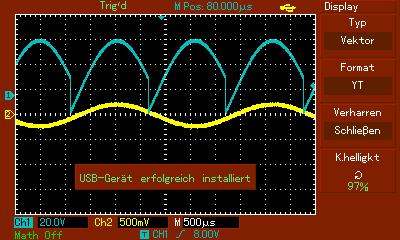
\includegraphics[width=0.8\textwidth]{bilder/0ohne.png}
        \caption{$\phi = \SI{0}{\degree}$.} 
        \label{fig:11}
    \end{minipage}
    \hfill
    \begin{minipage}{0.5\textwidth}
        \centering
        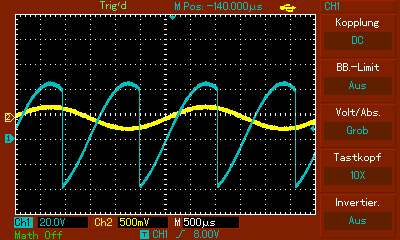
\includegraphics[width=0.8\textwidth]{bilder/45ohne.png}
        \caption{$\phi = \SI{45}{\degree}$.} 
        \label{fig:12}
    \end{minipage}
    \vspace{1cm}
    \vfill
    \begin{minipage}{0.5\textwidth}
        \centering
        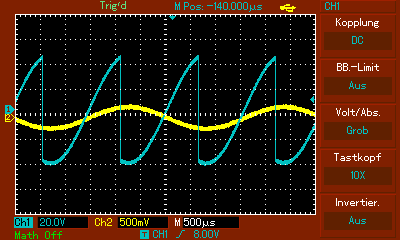
\includegraphics[width=0.8\textwidth]{bilder/90ohne.png}
        \caption{$\phi = \SI{90}{\degree}$.} 
        \label{fig:13}
    \end{minipage}
    \hfill
    \begin{minipage}{0.5\textwidth}
        \centering
        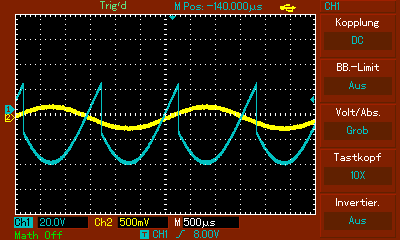
\includegraphics[width=0.8\textwidth]{bilder/135ohne.png}
        \caption{$\phi = \SI{135}{\degree}$.} 
        \label{fig:14}
    \end{minipage}
    \vspace{1cm}
    \vfill
    \begin{minipage}{0.5\textwidth}
        \centering
        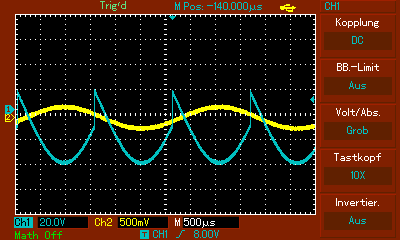
\includegraphics[width=0.8\textwidth]{bilder/180ohne.png}
        \caption{$\phi = \SI{180}{\degree}$.} 
        \label{fig:15}
    \end{minipage}
    \hfill
    \begin{minipage}{0.5\textwidth}
        \centering
        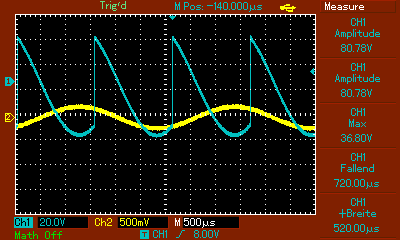
\includegraphics[width=0.8\textwidth]{bilder/240ohne.png}
        \caption{$\phi = \SI{240}{\degree}$.} 
        \label{fig:16}
    \end{minipage}
    \vspace{1cm}
    \vfill
    \begin{minipage}{0.5\textwidth}
        \centering
        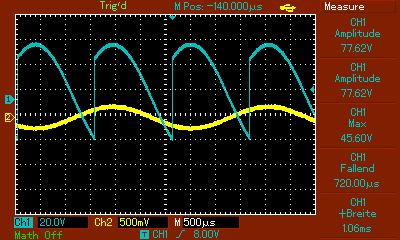
\includegraphics[width=0.8\textwidth]{bilder/300ohne.png}
        \caption{$\phi = \SI{300}{\degree}$.} 
        \label{fig:17}
    \end{minipage}
    \hfill
    \begin{minipage}{0.5\textwidth}
        \centering
        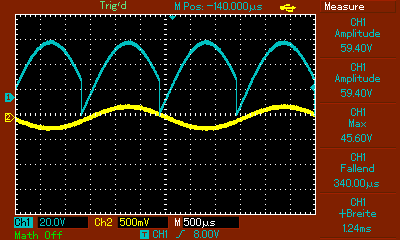
\includegraphics[width=0.8\textwidth]{bilder/360ohne.png}
        \caption{$\phi = \SI{360}{\degree}$.} 
        \label{fig:18}
    \end{minipage}
    \caption{Momentaufnahmen der phasenabhängigen Ausgangspannungen an einem Lock-In-Verstärker ohne Rauschen.}
\end{figure}

\subsection{Ausgangsspannung mit Rauschen}
